% \acsresetall
\chapter{Discussion}\label{chap:discussion}
\begin{flushright}{\slshape 
        Okay, well, sometimes science is more art than science, Morty. A lot of people don't get that.} \\ \medskip
        --- Rick Sanchez\\Rick and Morty, season 1, episode 6
\end{flushright}

\vspace{6cm}

The objective of this thesis was \objective.
This was based on the hypothesis that \MakeLowercase{\hypothesis} sleep stages, sleep events, and sleep disorders.
In this thesis, the system was realized using three models.
This chapter will touch on the results of three models as described in~\cref{chap:sleep-stage-classification,chap:sleep-event-detection,chap:classification-sleep-disorders}, and discuss aspects of including artificial intelligence in sleep clinics.

% \section{Sleep stage classification}
This thesis described methods for automatic sleep stage classification based on the manually annotated recordings according to the \ac{AASM} guidelines.
The outputs of this research theme were 
\begin{enumerate*}[label=\arabic*)]
    \item the \ac{MASSC} model, which yielded an accuracy of 84\% and a \cohen of 0.75 on a test set of 230 \acp{PSG} from \ac{WSC}, which increased to an accuracy of 87\% and \cohen of 0.80 using data from five different cohorts; and,
    \item the \ac{STAGES} model, which yielded an accuracy of 87\% and was found to be better than six independent scorers.
\end{enumerate*}
The main question is whether we should train sleep stage classifiers to perform as well as one or several human eyes, or, if we should let the classifiers rely more on the hidden fluctuations in the \ac{PSG} signals thereby allowing for more stages that are harder for the human eye to differentiate.
This has been the subject of other research groups in the past years. 
For example, \citeauthor{Stevner2019} modeled a combination of functional magnetic resonance imaging and \ac{EEG} whole-brain dynamics using a hidden Markov model approach in 57 subjects~\cite{Stevner2019}.
Their main findings identified multiple distinct whole-brain network states, and highlight that individual sleep stages can be characterized by several of these latent states; \eg they found that the \ac{W} and \ac{N1} stages are increasingly heterogeneous comprising multiple latent states, while \ac{N2} and \ac{N3} comprise only a few. 
Similar findings have also been found in patients expressing insomnia and Parkinson's disease, where a topic model was constructed in both cases using latent Dirichlet allocation of "words" created from the \ac{EEG}, \ac{EOG}, and \ac{EMG}, revealing that \ac{NREM} could be comprised of several topics~\cite{Koch2014, Christensen2019}, and that some individual topics\graffito{The same paper also found that individual signals possess different latent topics that describe various dissociations between sleep stages.} could describe a dissociated sleep stage \eg between \ac{N1} and \ac{N2}~\cite{Christensen2014}. 
Further evidence also points towards that local areas in the brain can be in different sleep stages~\cite{Koch2019}.
However, the clinical implications and utility of these findings are still unclear.

% \section{Detection of sleep events}
The second research theme concerned methods for automatic detection of sleep events focusing specifically on \acp{Ar}, \acp{LM}, and \ac{SDB} events.
The output of this research theme was the \ac{MSED} model, which yielded F1 scores of 0.704, 0.628, and 0.625 for \ac{Ar}, \ac{LM}, and \ac{SDB} detection, respectively, when tested on 1000 \acp{PSG}.
The \ac{MSED} model was also used in a study concerning \emph{transfer learning} in cases under the \emph{channel mismatch problem}, where it was demonstrated that the F1 score could be recovered effectively using a fine-tuning strategy.
The \ac{MSED} model was not tested against multiple scorers, as some studies have already proposed for \ac{LM} and \ac{Ar} detection~\cite{Carvelli2020, Brink-Kjaer2020}, which makes direct comparison of final performance difficult.
Indeed, this is true for any method based on \ac{AI}, which has prompted the development of benchmark datasets and competitions for computer vision applications, such as object recognition and localization in the ImageNet challenge~\cite{Russakovsky2015}.
This would be an important step forward in the future of computational sleep science.

% Other event types to characterize in the PSG that potentially correlate with these metrics
% \begin{itemize}
%     \item \printpublication{Carvelli2020}
%     \item \printpublication{Brink-Kjaer2020}
%     \item Hartmann S, Bruni O, Ferri R, Redline S, Baumert M. Characterization of cyclic alternating pattern during sleep in older men and women using large population studies. Sleep. 2020:1-9. doi:10.1093/sleep/zsaa016 \cite{Hartmann2020}
% \end{itemize}


% \section{Classification of sleep disorders}
The third research theme on methods for sleep disorder detection was mainly focused on central hypersomnias, in particular the detection of \ac{NT1}.
The development of the \ac{STAGES} algorithm, a machine learning model capable of classifying \ac{NT1} based on single-night \ac{PSG} with high sensitivity and specificity even without the addition of \hla typing or \ac{hcrt} serum levels, served as both the primary outcome and research contribution.
A secondary contribution relates to the identification of several novel \ac{PSG} features describing the dissociation between sleep stages, that was identified by the \ac{RFE} procedure.
Several research groups have found biomarkers describing increased sleep stage dissociation in narcolepsy~\cite{Sorensen2013b, Jensen2014, Christensen2015a, Olsen2017}, Parkinson's disease~\cite{Koch2014, Christensen2014, Christensen2016}, and insomnia~\cite{Christensen2019}, and the \ac{RFE} procedure could very likely help in revealing new biomarkers for various diseases.

A well-known effect in sleep medicine is the first night effect, wherein subjects experience more \ac{W} and less \ac{REM}~\cite{Agnew1966} during the first night of recording \ac{PSG}, which is not seen in the second night of recording.
Obviously, this will have an impact on the features extracted using the \ac{STAGES} model, but the extent of this impact needs further research.

Apart from the \ac{PSG} and \hla features, it is also possible that the addition of other types of research data would be of value.
It could be theorized that the addition of questionnaire data such as the Narcolepsy Severity Scale~\cite{Dauvilliers2020} or the Alliance Sleep Questionnaire would be beneficial for example in distinguishing between hypersomnias. 
This has been explored in other studies where \eg a digital sleep questionnaire was designed and used to classify and detect common societal sleep disturbances including insomnia, delayed sleep phase syndrome, insufficient sleep syndrome, and risk for obstructive sleep apnea~\cite{Schwartz2020}.

% Insert a sentence about other methods for clinical narcolepsy grading using \fullcite{Dauvilliers2020}~\cite{Dauvilliers2020}. 

% I don't know if this is needed somewhere~\fullcite{Adamantidis2020}.

% With an increased focus in the general population towards healthier sleep habits and the increased prevalence of sleep apnea, narcolepsy is not the only sleep disorder of interest for machine learning applications. 
% This This paper designed a digital sleep questionnaire to classify and detect common societal sleep disturbances including insomnia, delayed sleep phase syndrome, insufficient sleep syndrome, and risk for obstructive sleep apnea~\cite{Schwartz2020}.
% This paper focused on obstructive sleep apnea: \fullcite{Huang2020}~\cite{Huang2020}.

Our model consistently was able to distinguish \ac{NT1} from \ac{NT2} as well as IH, but not \ac{NT2} from IH, indicating a clear distinction between the two narcolepsy types and that IH and \ac{NT2} might be more related than previously thought, which is also being considered by other research groups~\cite{Fronczek2020}.
A panel consisting of European experts also recently reviewed the clinical findings for a future revision of the \ac{ICSD}, in which they recommend three new categorizations of central hypersomnias as narcolepsy, idiopathic hypersomnia, and idiopathic excessive sleepiness~\cite{Lammers2020}.

% \section{Accessible data for improving computational and clinical sleep science}
The main findings of this thesis argue that clinical sleep medicine can benefit from incorporating computational methods such as deep learning and machine learning.
% Condensing the main findings of this thesis into a single statement would be that clinical sleep medicine can benefit from incorporating computational methods such as deep learning or machine learning in general.
However, major challenges still face the sleep science community from wholly adopting automatic sleep analysis methods: % in the clinics, which has also been touched upon in this thesis. 
\begin{enumerate*}[label=\roman*)]
    \item accessibility of curated data remains a major obstacle, which is especially important for those researchers interested in applying or developing machine learning algorithms and statistical methods, 
    \item how to share clinical data in a safe and regulated manner compliant with GDPR specifications.
\end{enumerate*}
Several attempts have been made to address these issues; this thesis has relied heavily on data from the \ac{NSRR}, which contain several high-quality databases from research cohorts and clinical trials in a stream-lined format~\cite{Dean2016, Zhang2018}. 
\emph{PhysioNet} is another online resource containing vast amounts of freely accessible electrophysiological data, although the amount of sleep-related data is limited~\cite{Goldberger2000}. 

% \section{AI-based systems in the sleep clinic}
The \ac{AASM} Artificial Intelligence in Sleep Medicine Committee recently published a statement on behalf of the \ac{AASM} regarding the adoption and use of \ac{AI} in the sleep clinics.
Their official position of the \ac{AASM} is that electrophysiological data such as those originating from \ac{PSG} recordings, are well-suited for \ac{AI}-based analysis due to the volume and variability of data. 
They argue, that \ac{AI} analysis can add significant value by improving the efficiency of sleep labs, shifting focus away from manual analysis leading towards increased patient care, more rapid diagnosis and subsequent treatment~\cite{Goldstein2020a}.
However, they also emphasize that the goal of integrating \ac{AI}-based systems into clinical practice should be to augment rather than replace expert-based evaluations, and that full-scale adoption is complicated by logistics, limited transparency of \ac{AI}-based models, and ethical and regulatory issues~\cite{Goldstein2020b}.

The question then becomes if the field of sleep science and medicine is ready to move towards more automated sleep analysis?
In response to this question, \citeauthor{Lim2020} recently posed three advantages to automating sleep study scoring~\cite{Lim2020}.
The first advantage point is that sleep clinics will have consistent results on the same sleep studies for both clinical and research purposes, which potentially can be used for building new treatment protocols and build upon the collective findings.
The second mentioned advantage point is that automated sleep scoring will significantly reduce man-hours spent on \ac{PSG} analysis, which will free up precious time for physicians and technicians to focus on patient care.
The third and last mentioned advantage point is that automated sleep stage scoring has the potential to drive the field away from the current gold standard of scoring sleep stages and discover novel sleep stage characteristics in the brain.

% \section{New technical ways of analysing data}

% \begin{figure}[t]
%     \centering
%     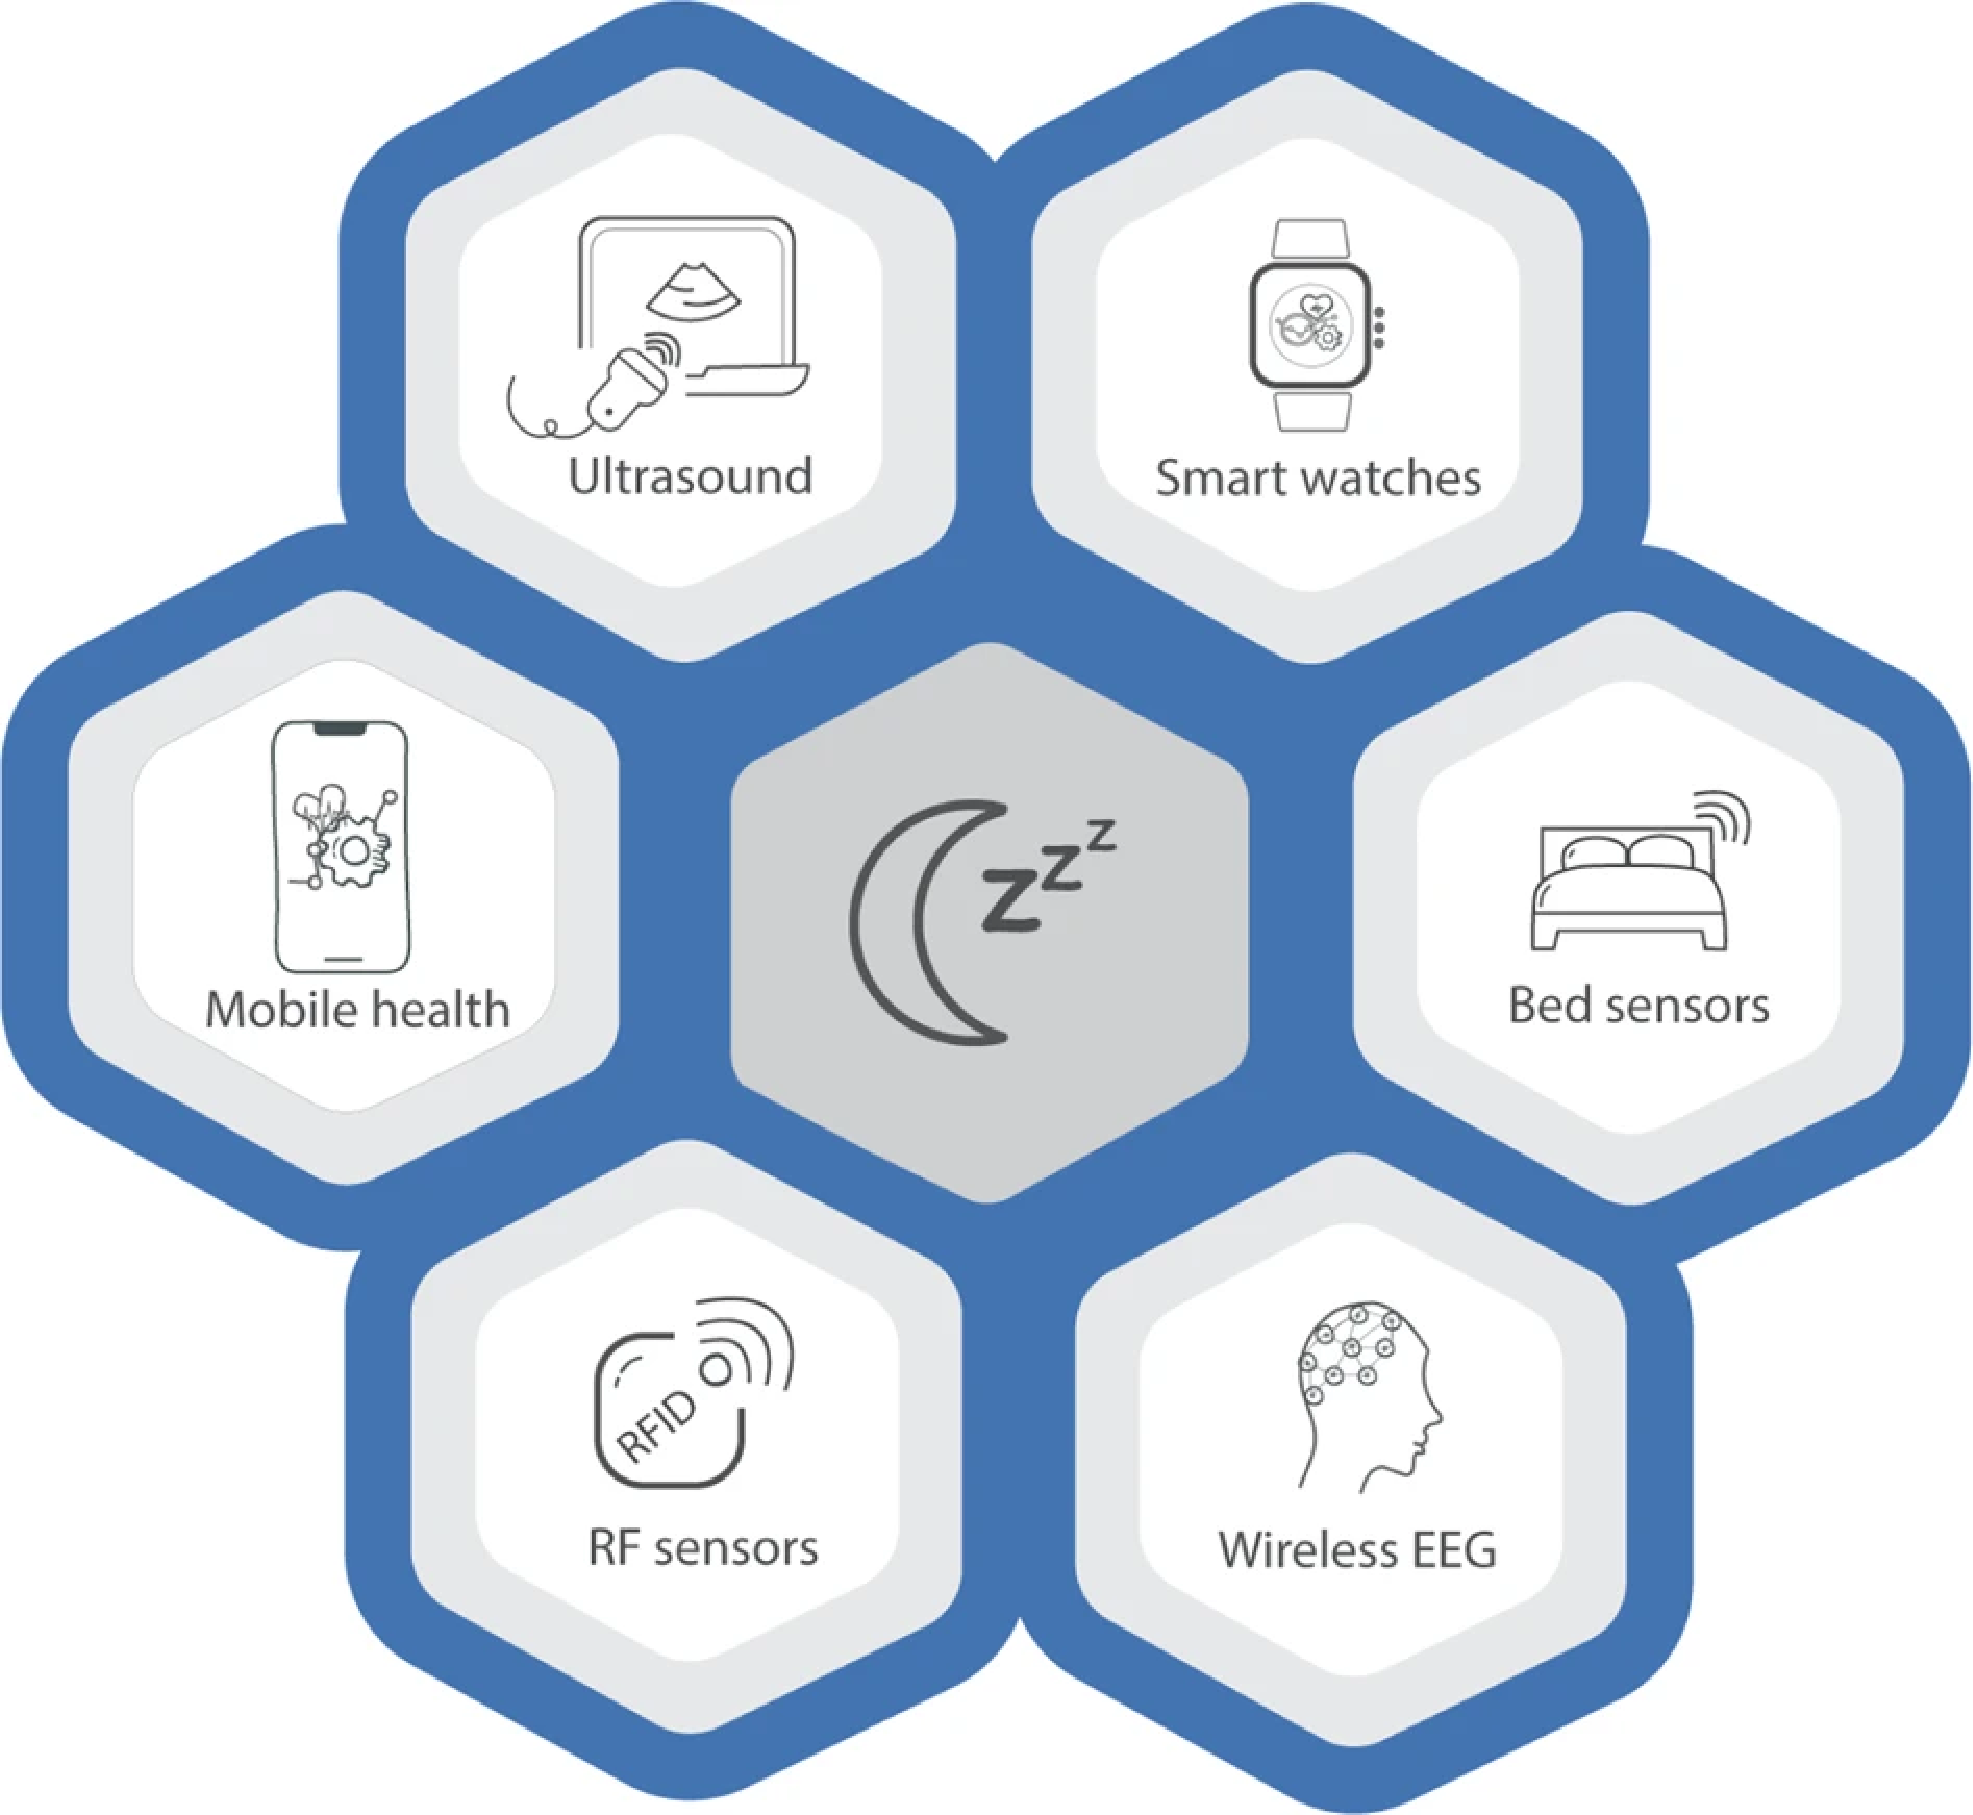
\includegraphics[width=\linewidth]{figures/introduction/npjFig2.pdf}
%     \caption[Emerging technologies in sleep analysis]{Emerging technologies for data acquisition in sleep analysis. Reprinted from~\cite{Perez-Pozuelo2020} under a Creative Commons Attributes 4.0 International License: \url{http://creativecommons.org/licenses/by/4.0/}.}
%     \label{fig:introduction:figure-01}
% \end{figure}

Moving beyond the \SI{30}{\second} scoring guidelines requires a drastic shift in methodology apart from a change in mindset.
The rise of machine learning, and in particular deep learning during the last decade, has prompted new and powerful ways to learn from data, that could be useful for developing future intelligent sleep analysis algorithms.
Coupled with the raw amount of data available from a sleep study with relatively few outcome labels, it seems highly probable that unsupervised learning will become increasingly popular for discovering new information about the processes and mechanisms of sleep.
Self-supervised representation learning is one such form of unsupervised learning, where a model is incentivized to define latent feature spaces given some data without any associated target labels.
The goal of defining such latent representations is to model the underlying data distribution for use in a later downstream task, which has been shown to work effectively for both audio, video and natural language processing domains~\cite{Oord2018, Henaff2019}.
Some studies have already been published made regarding the use of such self-supervised techniques for improving sleep stage scoring~\cite{Banville2019}.
The authors were able to effectively model the underlying data distribution of \ac{PSG} recordings to improve sleep stage scoring in cases where the amount of data was not sufficient to effectively train traditional machine learning or deep learning-based models~\cite{Banville2019}.
As this type of modeling is, in a sense, agnostic to the \graffito{A downstream task is a secondary task that a model is not originally trained to complete.}downstream task at hand, this could be a potential avenue for future research aiming to design "one-shot-analysis"-type\graffito{This could \eg be a model that is able to detect micro-sleep events, predict sleep disorders, recommend treatment plans, \etc.} models, which is capable of doing everything at once.

However, it is naïve to think that clinician experience would be redundant in the future of clinical sleep medicine due to automated systems.
Semi-supervised learning systems could benefit from having both the robustness and objectivity of the machine, as well as the expertise and flexibility of a trained professional.
% This has already been shown in studies, where the manual scorings were augmented with deep learning-based systems for sleep staging.
Recently, \textit{explainable \ac{AI}} has emerged as a possible tool for further analysis of deep learning models~\cite{Samek2019}, and could also offer new insight into sleep analysis~\cite{Vilamala2017}.

% \begin{itemize}
%     \item Interpretability (explainable AI)
%     \item supervised vs. semi- and unsupervised learning (\eg 30 s epoch debate).
% \end{itemize}

% \section{Sleep stage discussion points}
% \begin{itemize}
%     \item Something about non-contact sleep stage estimation \eg using radar based systems.
%     \item Non-PSG, commercial systems:
%     \begin{itemize}
%         \item Roberts DM, Schade MM, Mathew GM, Gartenberg D, Buxton OM. Detecting Sleep Using Heart Rate and Motion Data from Multisensor Consumer-Grade Wearables, Relative to Wrist Actigraphy and Polysomnography. Sleep. 2020. doi:10.1093/sleep/zsaa045 \cite{Roberts2020}
%         \item \fullcite{Depner2019}
%         \item \fullcite{Fonseca2020}~\cite{Fonseca2020}
%         \item \fullcite{Sun2019}~\cite{Sun2019}
%     \end{itemize}
% \end{itemize}

% Papers to include:
% \begin{itemize}
%     \item Lim DC, Mazzotti DR, Sutherland K, et al. Reinventing Polysomnography in the Age of Precision Medicine. Sleep Med Rev. 2020. doi:10.1016/j.smrv.2020.101313
%     \item Fiorillo L, Puiatti A, Papandrea M, et al. Automated sleep scoring: A review of the latest approaches. Sleep Med Rev. 2019;48:101204. doi:10.1016/j.smrv.2019.07.007
% \end{itemize}


